%compile with pdflatex on papeeria

\documentclass[a4paper,12pt]{article}
\usepackage{fancyhdr}
\usepackage{fancyheadings}
\usepackage[ngerman,german]{babel}
\usepackage{german}
\usepackage[utf8]{inputenc}
%\usepackage[latin1]{inputenc}
\usepackage[active]{srcltx}
%\usepackage{algorithm}
%\usepackage[noend]{algorithmic}
\usepackage{amsmath}
\usepackage{amssymb}
\usepackage{amsthm}
\usepackage{bbm}
\usepackage{enumerate}
\usepackage{graphicx}
\usepackage{ifthen}
\usepackage{listings}
\usepackage{enumitem}
%\usepackage{struktex}
\usepackage{hyperref}
\usepackage{tikz}


\pagenumbering{gobble}

%%%%%%%%%%%%%%%%%%%%%%%%%%%%%%%%%%%%%%%%%%%%%%%%%%%%%%
%%%%%%%%%%%%%% EDIT THIS PART %%%%%%%%%%%%%%%%%%%%%%%%
%%%%%%%%%%%%%%%%%%%%%%%%%%%%%%%%%%%%%%%%%%%%%%%%%%%%%%
\newcommand{\Fach}{Tägliche Übung aus der Mathematik (A) - Musterlösung}
\newcommand{\Name}{}
\newcommand{\datum}{}
\newcommand{\Matrikelnummer}{}
\newcommand{\Semester}{Q12/1}
\newcommand{\Uebungsblatt}{} %  <-- UPDATE ME
%%%%%%%%%%%%%%%%%%%%%%%%%%%%%%%%%%%%%%%%%%%%%%%%%%%%%%
%%%%%%%%%%%%%%%%%%%%%%%%%%%%%%%%%%%%%%%%%%%%%%%%%%%%%%

\setlength{\parindent}{0em}
\topmargin -1.0cm
\oddsidemargin 0cm
\evensidemargin 0cm
\setlength{\textheight}{9.2in}
\setlength{\textwidth}{6.0in}


\newcounter{aufgabencounter}
\newcommand{\aufgabeNr}{\stepcounter{aufgabencounter}{\theaufgabencounter}}


%%%%%%%%%%%%%%%
%% Aufgaben-COMMAND
\newcommand{\Aufgabe}{
  {
  \vspace*{0.5cm}
  \textsf{\textbf{Aufgabe \aufgabeNr}}
  \vspace*{0.2cm}
  
  }
}

\lstset{ %
language=java,
basicstyle=\footnotesize\tt,
showtabs=false,
tabsize=2,
captionpos=b,
breaklines=true,
extendedchars=true,
showstringspaces=false,
flexiblecolumns=true,
}

\title{Übungsblatt \Uebungsblatt{}}
\author{\Name{}}

\begin{document}
\thispagestyle{fancy}
%\lhead{\sf \large \Fach{} \\ %\small \Name{} - \Matrikelnummer{}
\lhead{\sf \large \Fach{} %\small \Name{} - \Matrikelnummer{}
}

\begin{figure}[h!tp]
\vspace*{-0.66cm}
\makebox[\textwidth][c]{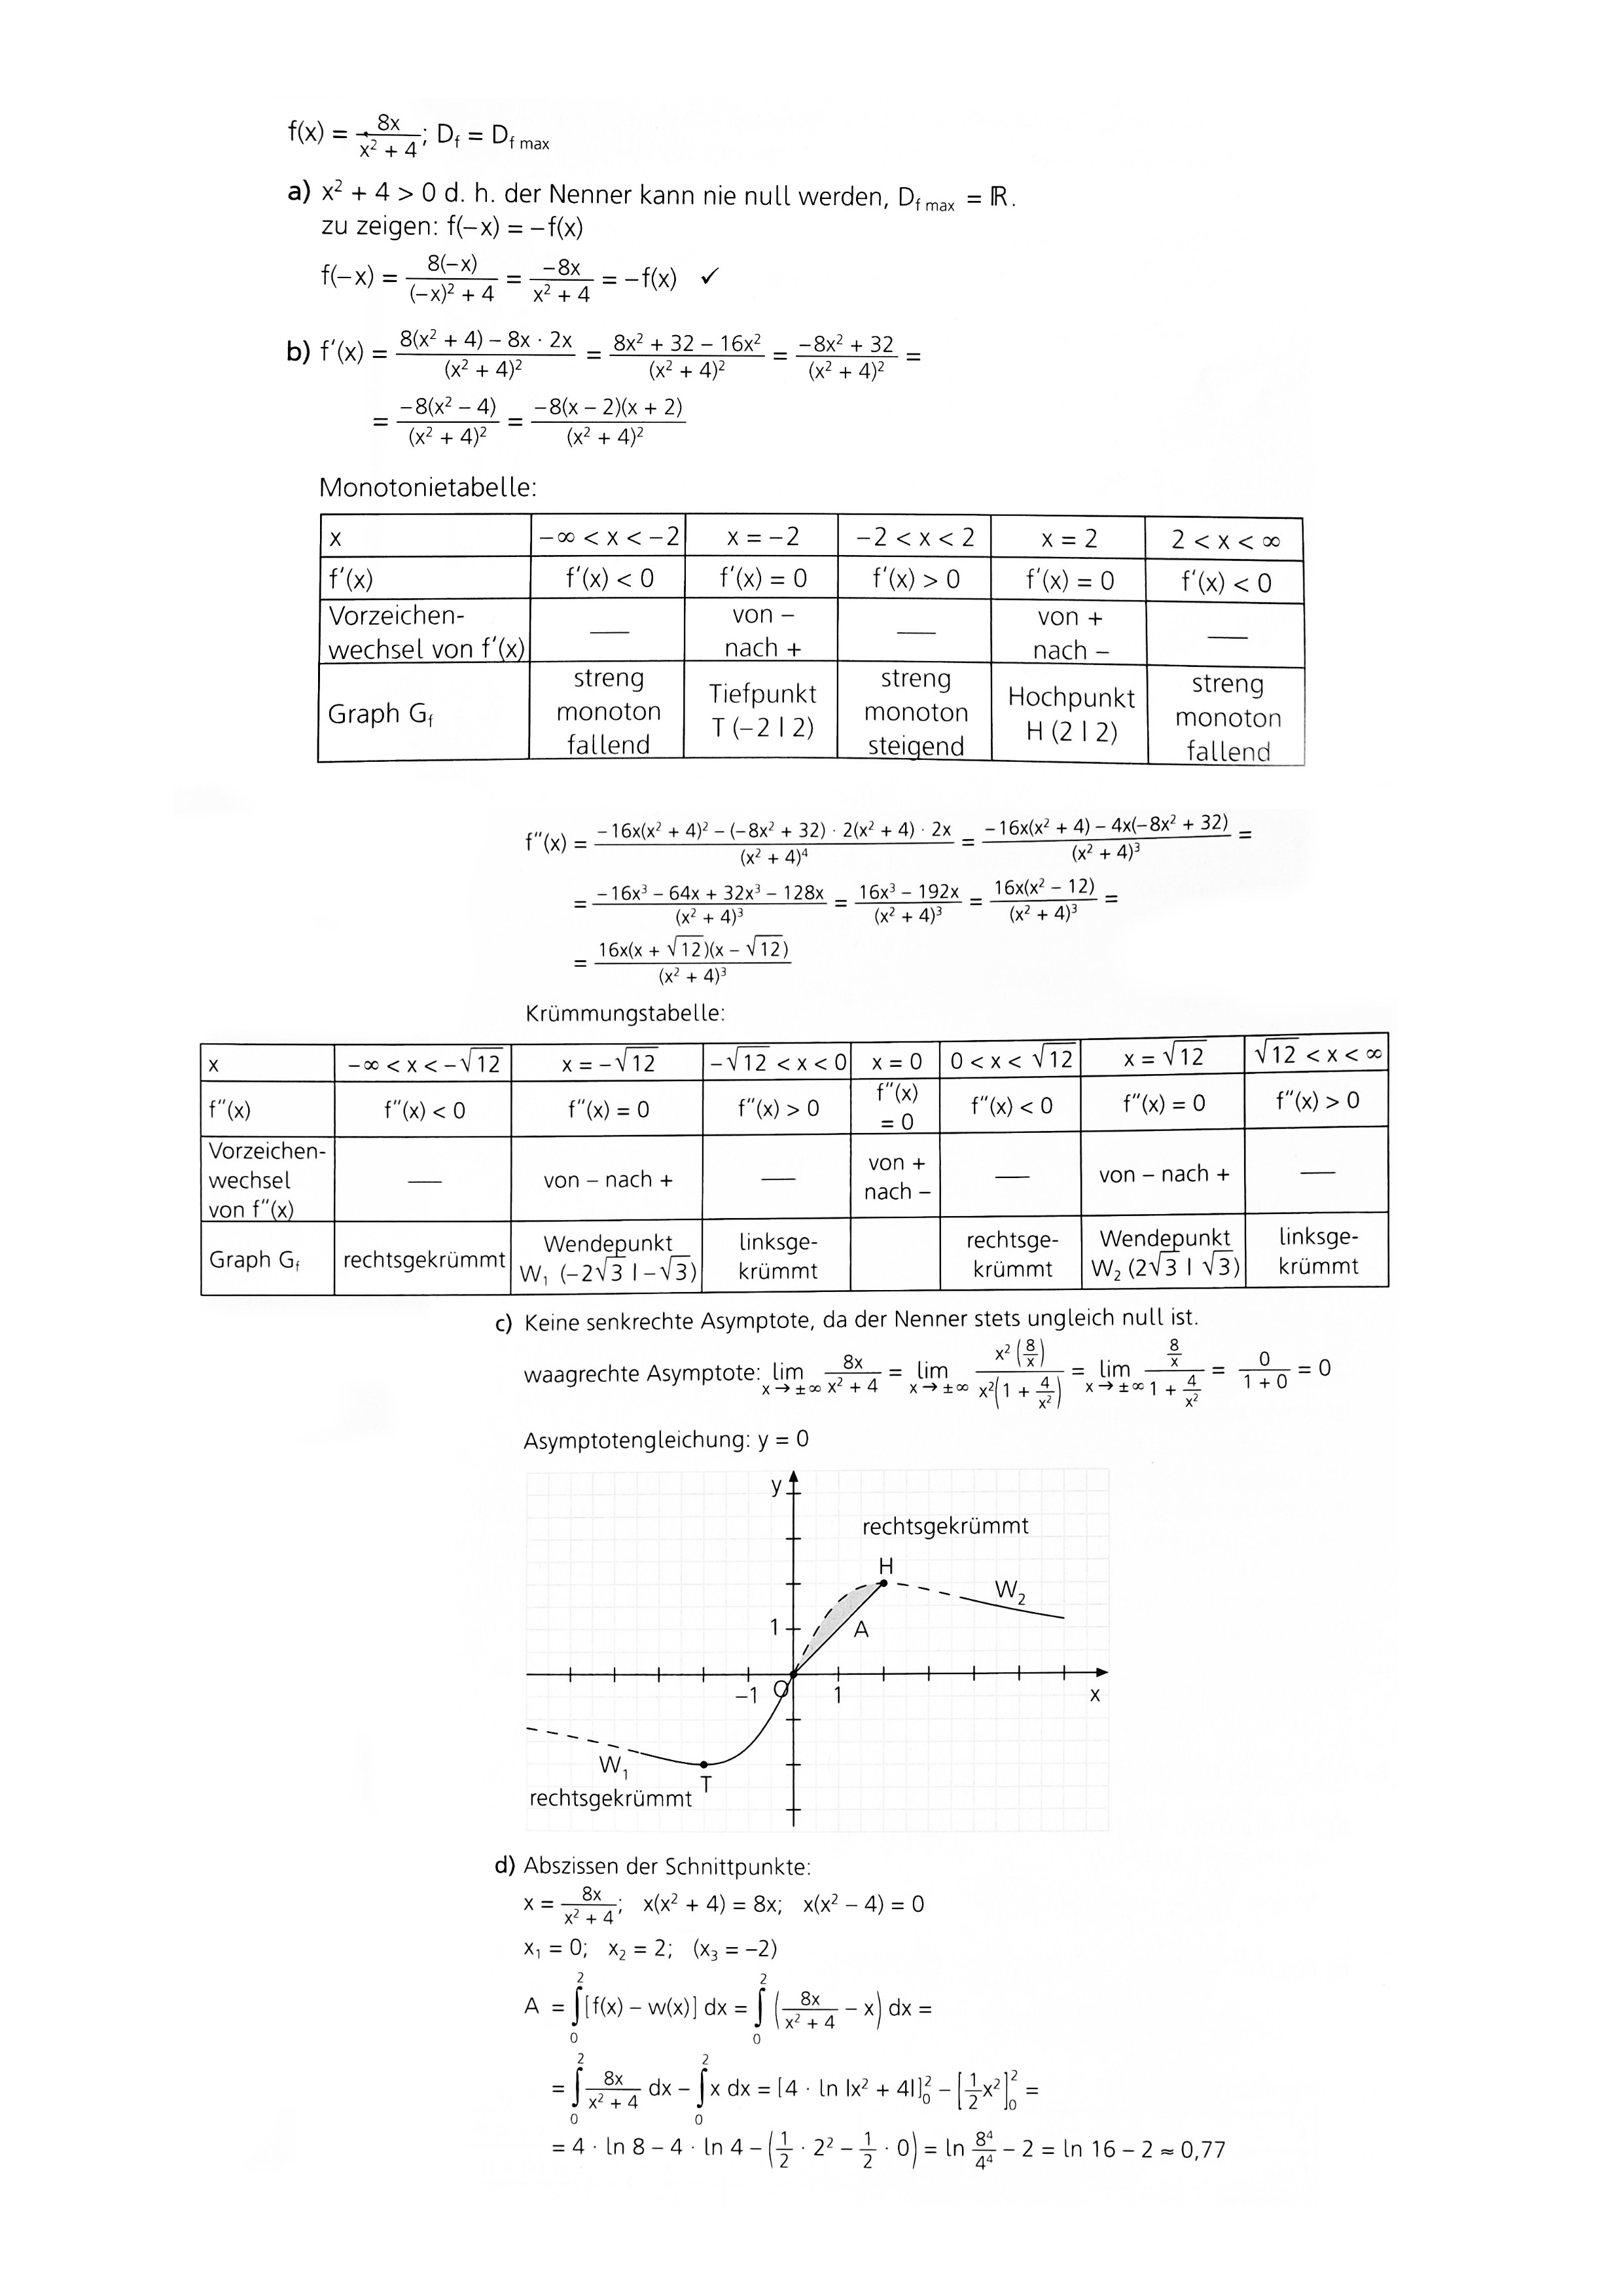
\includegraphics[width=1.3\textwidth]{Q12_TÜ_Integrale_Anwendung_MusterLösung.jpg}}
\end{figure}

%  \begin{figure}[ht]
%    \centering
%    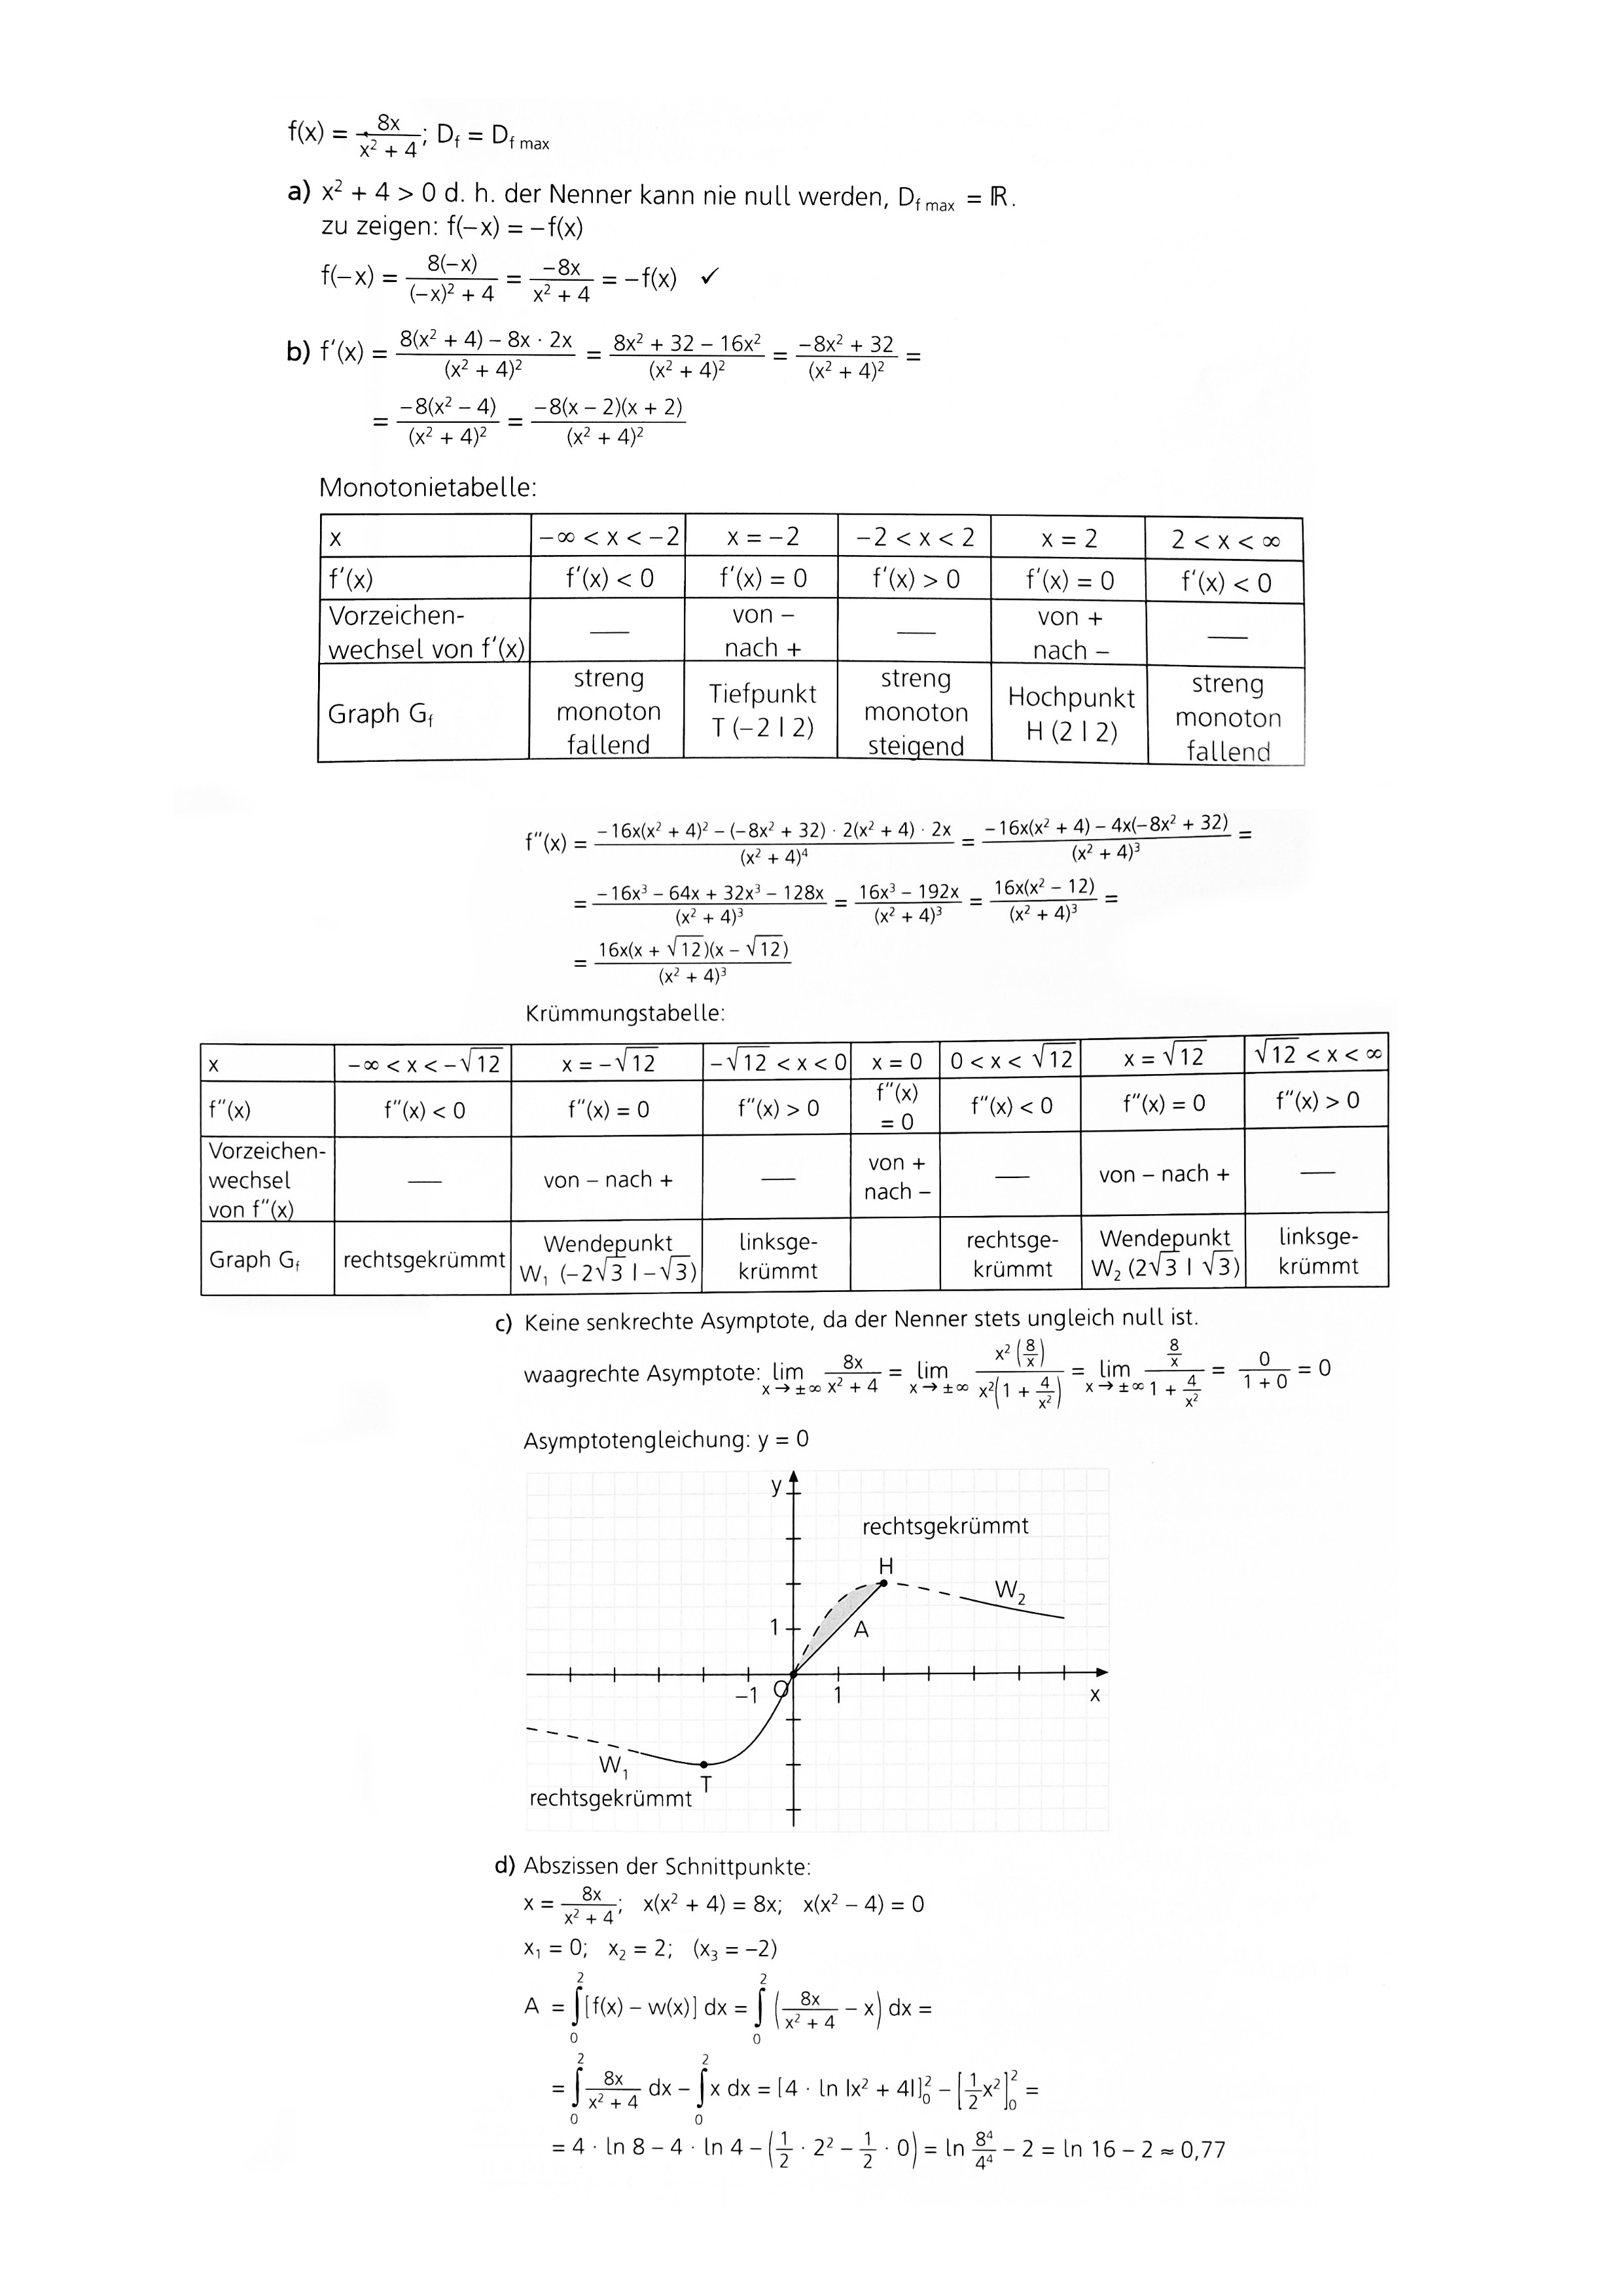
\includegraphics[width=0.84\columnwidth]{Q12_TÜ_Integrale_Anwendung_MusterLösung.jpg}
%    %\caption{A boat.}
%    %\label{fig:boat1}
%  \end{figure}

%%%%%%%%%%%%%%%%%%%%%%%%%%%%%%%%%%%%%%%%%%%%%%%%%%%%%%
%%%%%%%%%%%%%%%%%%%%%%%%%%%%%%%%%%%%%%%%%%%%%%%%%%%%%%
\end{document}
